
\clearpage
\section{La configuration}

\begin{wrapfigure}[14]{l}{6.5cm}   % [x] Wie manche Zeile soll sich um die Grafik "brechen"
  \vspace{-35pt}      % Grundwert war 20; mit 30 schön oben beim Text ausgerichtet
  \begin{center}
    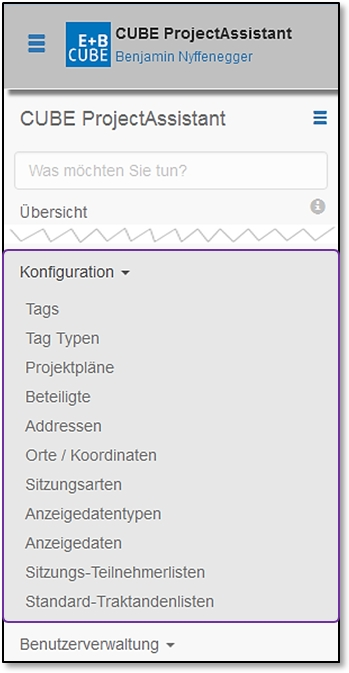
\includegraphics[width=1\linewidth]{../chapters/13_Konfigurationen/pictures/13_Menu_Konfiguration.jpg}
  \end{center}
  \vspace{-20pt}
  \caption{Configurer CUBE PA}
  \vspace{-10pt}
\end{wrapfigure}

En règle générale, la configuration est effectuée par un administrateur ou un 'power user' qui a été entraîné pour ce rôle. Pour cette raison, ce chapitre ne présente pas le processus de configuration dans les détails. En cas de doute, il est conseillé de contacter le support CUBE PA pour toute question ouverte ou incertitude (voir chapitre \ref{bkm:Ref443502661}).

\vspace{\baselineskip}

Dans le menu à gauche, sélectionnez l'élément de menu 'Configuration'. Les sous-éléments qui s'affichent sont brièvement présentés ci-dessous.

\vspace{1.5cm} 

Pour les utilisateurs qui ne disposent pas des droits d'accès nécessaires, ces éléments ne seront pas affichés. \\

\vspace{3.5cm}  

\textbf{Aperçu des possibilités de configuration :}

\vspace{\baselineskip}

\begin{itemize}
\item
\textbf{Tags} : Les tags (étiquettes) peuvent être saisis ici et classifiés par 'types de tag'. Les tags sont utilisés dans la gestion de documents, par exemple pour désigner les documents selon leur thème afin de pouvoir les retrouver plus facilement. 
Les tags 'Projets / Sous-projets' sont utilisés à plusieurs endroits dans CUBE PA (par exemple dans la gestion de séances, et la fonction de procuration).
\item
\textbf{Types de tag} : Des types de tag (ou catégories) selon lesquelles les tags peuvent être classifiés 
peuvent être définis ici.
\item
\textbf{Planning détaillé} : Plusieurs plannings (par exemple des échéanciers détaillés) peuvent être créés ici. Les plannings détaillés peuvent être sélectionnés et importés séparément par le moyen de la fonction d'importation (importer des données d'échéancier).
\item
\textbf{Participants} : Les participants peuvent être créés ici pour être utilisés dans plusieurs processus de CUBE PA. Les participants sont pour la plupart des entreprises, des comités, ou d'autres unités d'organisation. Selon leur fonction dans le projet, les participants peuvent être désignés comme 'Entreprise', 'Client', 'Mandataire', 'Comité', etc. Cette désignation détermine à quels endroits les participants concernés apparaissent dans les champs de sélection.
\item
\textbf{Adresses} : Des adresses, qui peuvent être utilisées comme lieux de séances ou lieux de procès-verbaux de séances, peuvent être saisies ici.
\item
\textbf{Lieu / Coordonnées}: Ces saisies font référence à des lieux liés à des projets, par exemple des passages à niveau, des gares, etc., qui peuvent être liés à Google Maps. Ces lieux / coordonnées prédéfinis facilitent l'attribution de coordonnées aux documents dans le classement de documents. Leur utilisation est cependant facultative. Des coordonnées non définies à l'avance peuvent également être attribuées à des documents.
\item
\textbf{Types de séances} : Les différents types de séances et responsabilités peuvent être gérés ici. Dans la version actuelle de CUBE PA, la gestion des droits d'accès pour les séances se fait uniquement dans la gestion des utilisateurs.
\item
\textbf{Types de données d'affichage et données d'affichage} : Des documents contenant des informations importantes et qui doivent facilement accessibles aux utilisateurs peuvent être classés ici. Ceci se fait à travers des saisies supplémentaires configurables dans le menu, ou types de données d'affichage. Pour chaque type de donnée d'affichage, l'élément de menu sous lequel la saisie doit apparaître peut être spécifié (par exemple sous la gestion des séances ou la gestion de la qualité). Les documents en soi sont appelés données d'affichage. 
Plusieurs données d'affichage peuvent être classifiés sous le même type de donnée d'affichage. Il est également possible de désigner une personne comme responsable pour une donnée d'affichage spécifique. Il est conseillé d'utiliser cette fonction avec modération, afin de ne pas surcharger le menu. La fonction peut par exemple être utilisée pour afficher un échéancier complet s'il est disponible uniquement sous forme de fichier Excel et pas sous forme de ficher MS Project.
\item
\textbf{Listes de participants à la séance} : Des liste de participants prédéfinies pour des séances peuvent être préparées ici. Vous pouvez aussi définir si les participants choisis sont sur la liste de distribution ou pas. Les listes peuvent ensuite être sélectionnées lors de la création d'invitations à des séances.
\item
\textbf{Ordres du jour standards} : Des éléments d'ordre du jour récurrents peuvent être prédéfinis ici et ensuite choisis lors de la création d'une séance.
\end{itemize}

\vspace{\baselineskip}

Les différents masques de saisie pour les éléments de configuration décrits ci-dessus sont brièvement présentés ci-dessous. Pour des informations plus détaillées ou d'autre informations, veuillez contacter le support CUBE PA : {\color{red} cube.support@emchberger.ch}

\subsection{Tags}

De nouveaux tags peuvent être créés, visualisés, ou modifiés ici.

\begin{figure}[H]
\center{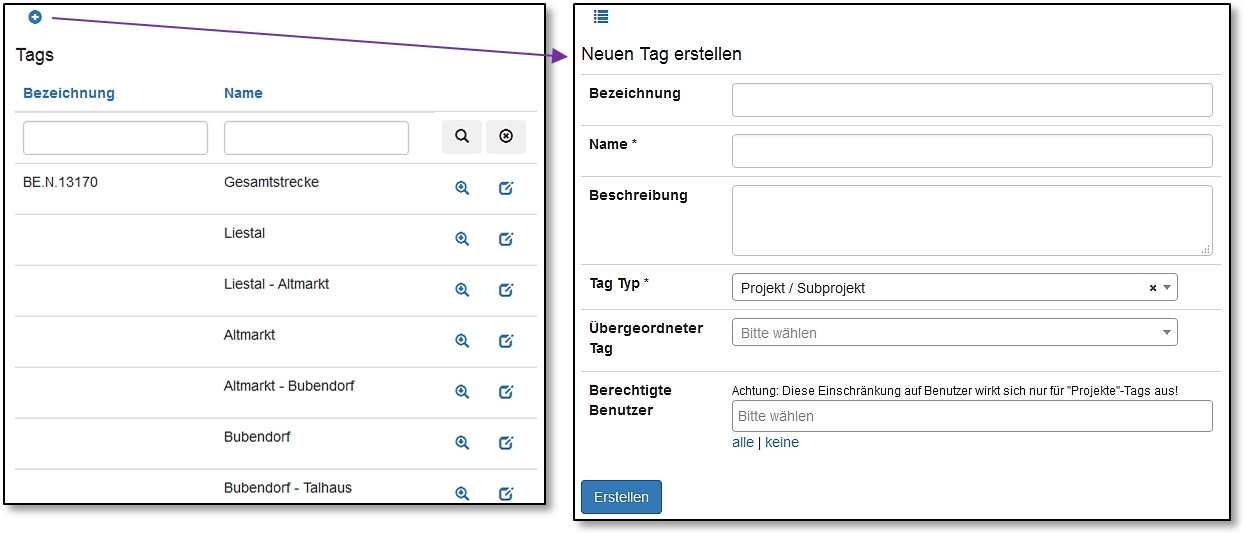
\includegraphics[width=1\linewidth]{../chapters/13_Konfigurationen/pictures/13-1_TagsHinzufuegen.jpg}}
\caption{Saisir un nouveau tag}
% \label{fig:speciation}
\end{figure}

La 'Désignation' est pour l'instant utilisée pour les projets / sous-projets uniquement. Le numéro de projet peut être saisi dans ce champ.

\vspace{\baselineskip}

Le 'Nom' (champ obligatoire) sera utilisé partout dans CUBE PA pour le tag correspondant.

\vspace{\baselineskip}

Les tags doivent être classifiés sous un type de tag (voir chapitre \ref{bkm:Ref444100222}).

\vspace{\baselineskip}

Il est possible de mettre en place une hiérarchie de tags. Pour ce faire, le champ 'Tags supérieurs' est à remplir. Plusieurs tags peuvent être attribués au même tag supérieur.

\vspace{\baselineskip}

Dans les prochaines versions de CUBE PA, il sera possible d'inclure les tags inférieurs dans le filtrage de tags et les fonctions de recherche. Dans la version actuelle de CUBE PA la hiérarchie de tags est encore limitée.

\vspace{\baselineskip}

Remarque : La sélection d'utilisateurs autorisés est uniquement valable pour les tags de projets (voir remarque).

\subsection{Types de tag}
\label{bkm:Ref444100222}
Comme les tags constituent un outil universel dans CUBE PA, des catégories de tag, appelées types de tag, peuvent être définies. \newline

Ceci permet de classer les documents avec des tags par rapport à différents critères. Les critères incluent par exemple le type de document ou le sujet. La catégorie 'Projet / Sous-projet' est également enregistrée comme type de tag et est utilisée quand la case 'est projet' est cochée. Ceci permet la sélection de tags de cette catégorie là ou la classification sous un sous-projet est désirée (par exemple dans les séances ou les acquisitions). \newline

Les types de tag qui doivent être utilisés pour la catégorisation de documents peuvent être utilisés quand la case 'est tag de document' est cochée. La séquence d'affichage des types de tag peut être définie en saisissant des numéros dans le champ 'Position'. L'ordre est croissant.

\begin{figure}[H]
\center{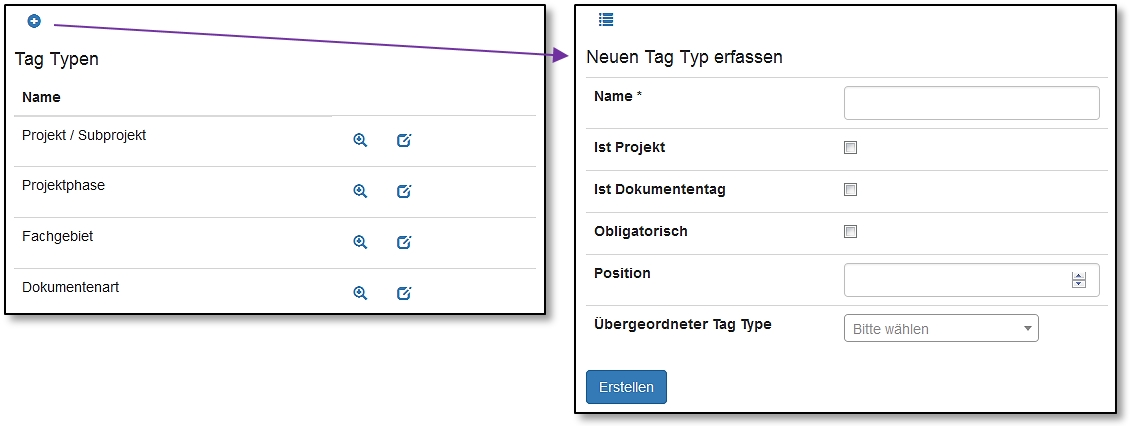
\includegraphics[width=1\linewidth]{../chapters/13_Konfigurationen/pictures/13-2_TagTypenHinzufuegen.jpg}}
\caption{Créer un nouveau type de tag}
% \label{fig:speciation}
\end{figure}\pagebreak

\subsection{Plannings détaillés}

Vous pouvez créer plusieurs plannings détaillés (par exemple échéancier détaillé, échéancier détaillé pour sous-projets), pour lesquels des saisies différentes peuvent être importées avec la fonction d'importation de données d'échéanciers.

\begin{figure}[H]
\center{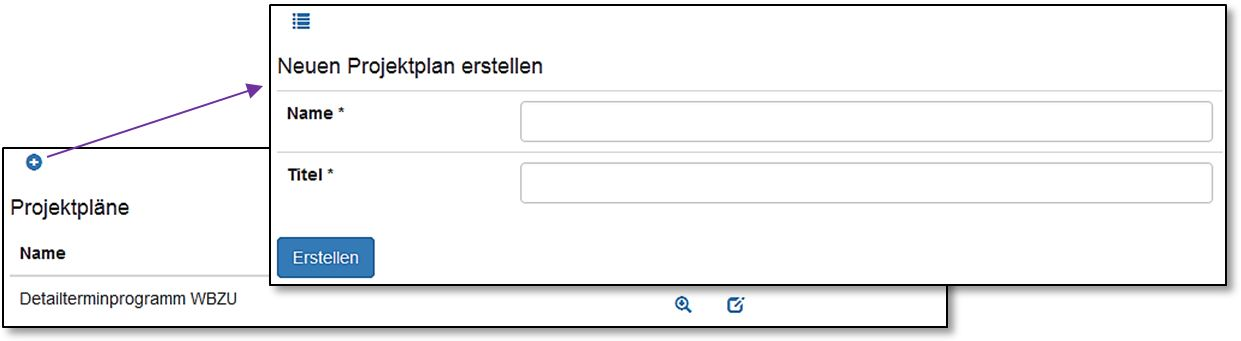
\includegraphics[width=1\linewidth]{133_ProjektplaeneHinzufuegen.jpg}}
\caption{Saisir un nouveau planning détaillé}
% \label{fig:speciation}
\end{figure}

Tous les plannings détaillés saisis sont listés ici. Vous pouvez les visualiser ou les modifier dans l'aperçu détaillé. De nouvelles saisies peuvent également être créées sous cet élément de configuration.

\subsection{Participants}

\begin{wrapfigure}[11]{r}{6cm}
\vspace{-25pt}
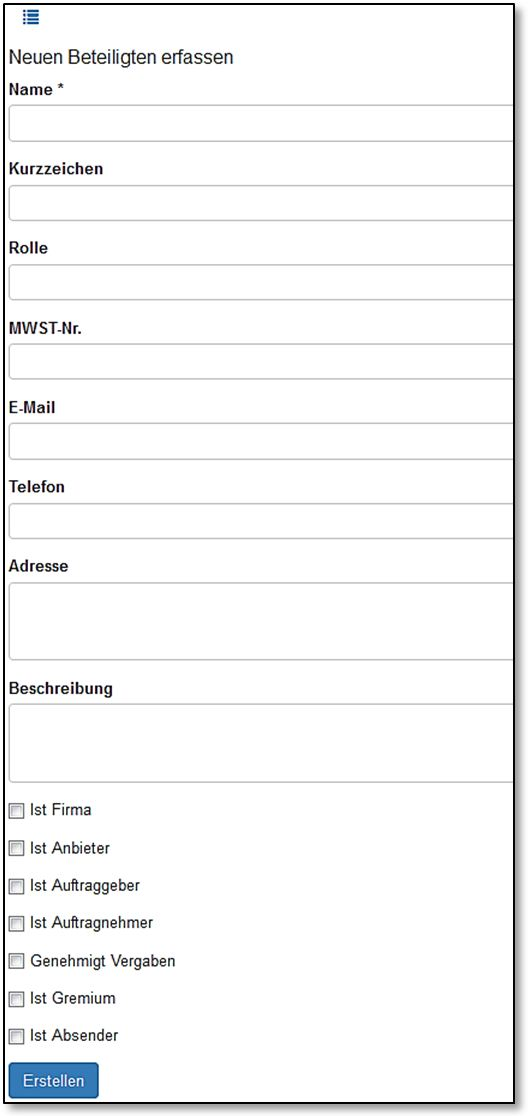
\includegraphics[height=150mm]{134_BeteiligteHinzufuegen.jpg}
% \caption{Status ändern}
\end{wrapfigure}

Les participants impliqués dans un projet peuvent être saisis ici et attribués différents 'rôles'.

\begin{center}
\hspace{-15pt}   
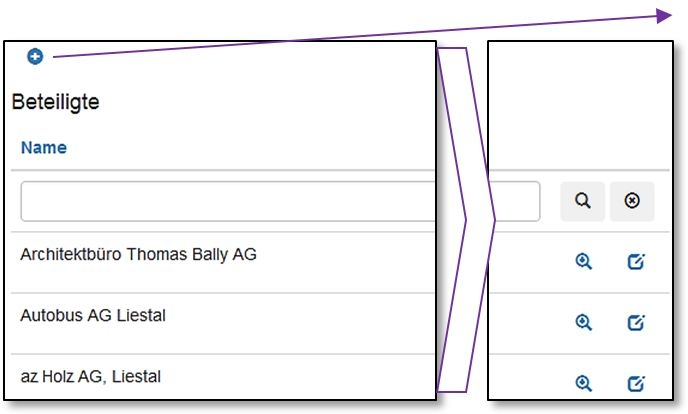
\includegraphics[width=.9\linewidth]{../chapters/13_Konfigurationen/pictures/13-4_Beteiligte.jpg}
\end{center}

Le champ 'Rôle' est un champ de texte libre dans lequel le rôle du participant au sein d'un projet peut être défini.

\vspace{\baselineskip}

Les cases 'est entreprise', 'est client', etc. permettent au participant d'être référencé et disponible pour sélection dans CUBE PA. Par exemple, si la case '[x] est entreprise' est cochée, le participant sera inclus dans les champs de sélection / menus déroulants 'entreprise'.

\vspace{\baselineskip}
\vspace{\baselineskip}
\vspace{\baselineskip}

% -->>> Wenn \clearpage löschen > Achtung Formatierung zu vorhergehendem Bild beachten -> allenfalls \clearpage bestehen lassen
% \clearpage
\subsection{Adresses}

Les adresses sont en règle générale des salles de conférences. Des lieux (sans fonction de salle de conférences) peuvent également être saisis. La case 'est salle de conférence' doit être cochée ou laissée vide selon le cas.

\begin{figure}[H]
\center{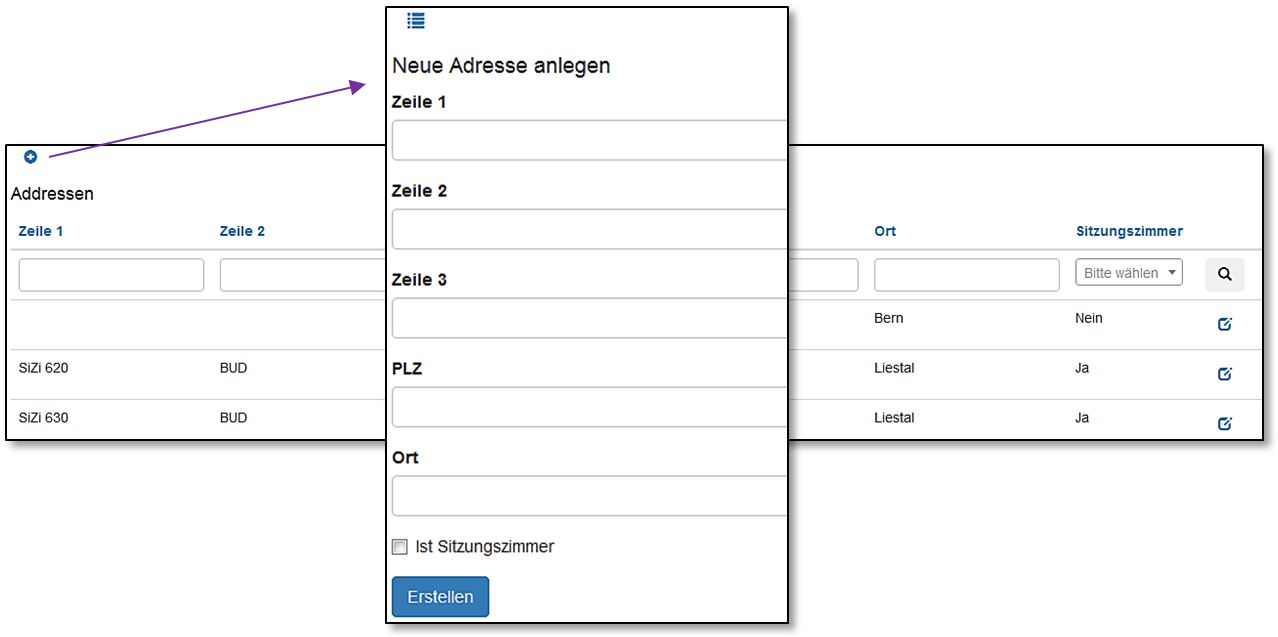
\includegraphics[width=1\linewidth]{135_AdresseHinzufuegen.jpg}}
\caption{Saisir une nouvelle adresse}
% \label{fig:speciation}
\end{figure}

\subsection{Lieu / Coordonnées}

Ces saisies font référence à des lieux liés à un projet, par exemple des passages à niveau, des gares, etc. qui peuvent être liés à Google Maps. Cliquez sur le repère pour afficher la position dans Google Maps.

\begin{figure}[H]
\center{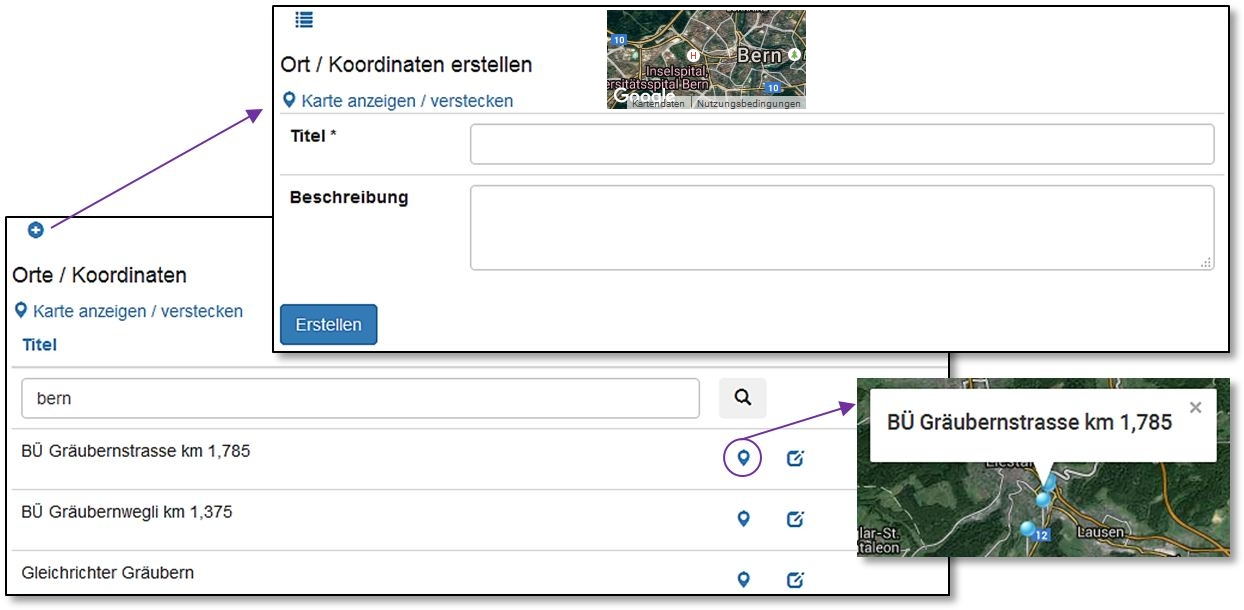
\includegraphics[width=1\linewidth]{../chapters/13_Konfigurationen/pictures/13-6_KoordinatenHinzufuegen.jpg}}
\caption{Saisir lieu / coordonnées}
% \label{fig:speciation}
\end{figure}

\clearpage
\subsection{Types de séances}

Les différents types de séances et les utilisateurs autorisés à ces séances sont créés ici.

\vspace{\baselineskip}


Vous pouvez prédéfinir la 'Direction' et le 'Remplaçant' pour un type de séance et l'adapter 
plus tard si nécessaire.

\begin{figure}[H]
\center{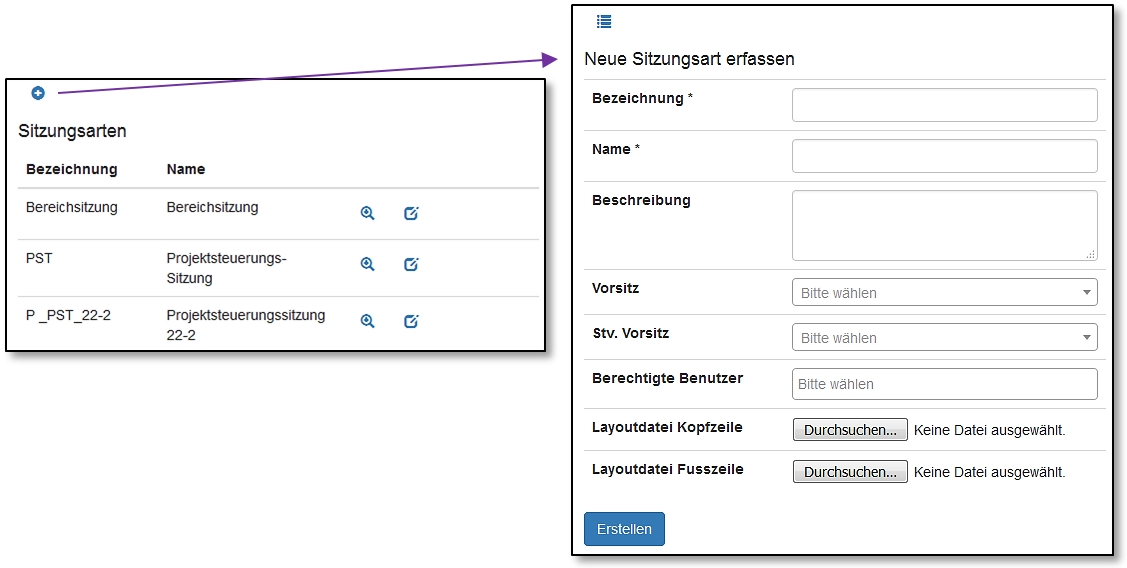
\includegraphics[width=1\linewidth]{../chapters/13_Konfigurationen/pictures/13-7_SitzungsartHinzufuegen.jpg}}
\caption{Saisir un nouveau type de séance}
% \label{fig:speciation}
\end{figure}

\subsection{Types de données d'affichage et données d'affichage}

Des documents contenant des informations importantes et qui doivent facilement accessibles aux utilisateurs peuvent être classés ici. Ceci se fait à travers des saisies supplémentaires configurables dans le menu, ou types de données d'affichage. Pour chaque type de donnée d'affichage, l'élément de menu sous lequel la saisie doit apparaître peut être spécifié (par exemple sous la gestion des séances ou la gestion de la qualité). Les documents en soi sont appelés données d'affichage. Plusieurs données d'affichage peuvent être classifiés sous le même type de donnée d'affichage. Il est également possible de désigner une personne comme responsable pour une donnée d'affichage spécifique. Il est conseillé d'utiliser cette fonction avec modération, afin de ne pas surcharger le menu. La fonction peut par exemple être utilisée pour afficher un échéancier complet s'il est disponible uniquement sous forme de fichier Excel et pas sous forme de ficher MS Project.

\vspace{\baselineskip}

Le nom d'un type de donnée d'affichage est à garder aussi concis et court que possible. Il sera affiché dans le menu sous l'élément de menu choisi. Pour cette raison, un long nom ou une phrase sont à éviter.

\begin{figure}[H]
\center{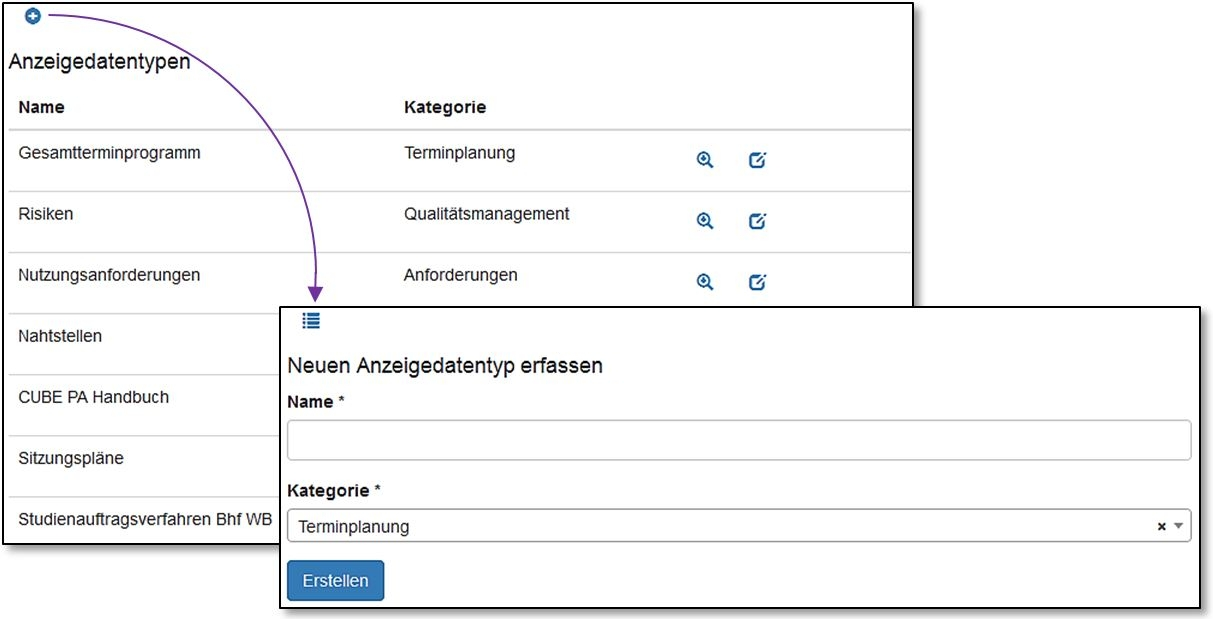
\includegraphics[width=1\linewidth]{138_AnzeigetypenErfassen.jpg}}
\caption{Saisir un nouveau type de données d'affichage}
% \label{fig:speciation}
\end{figure}

\begin{figure}[H]
\center{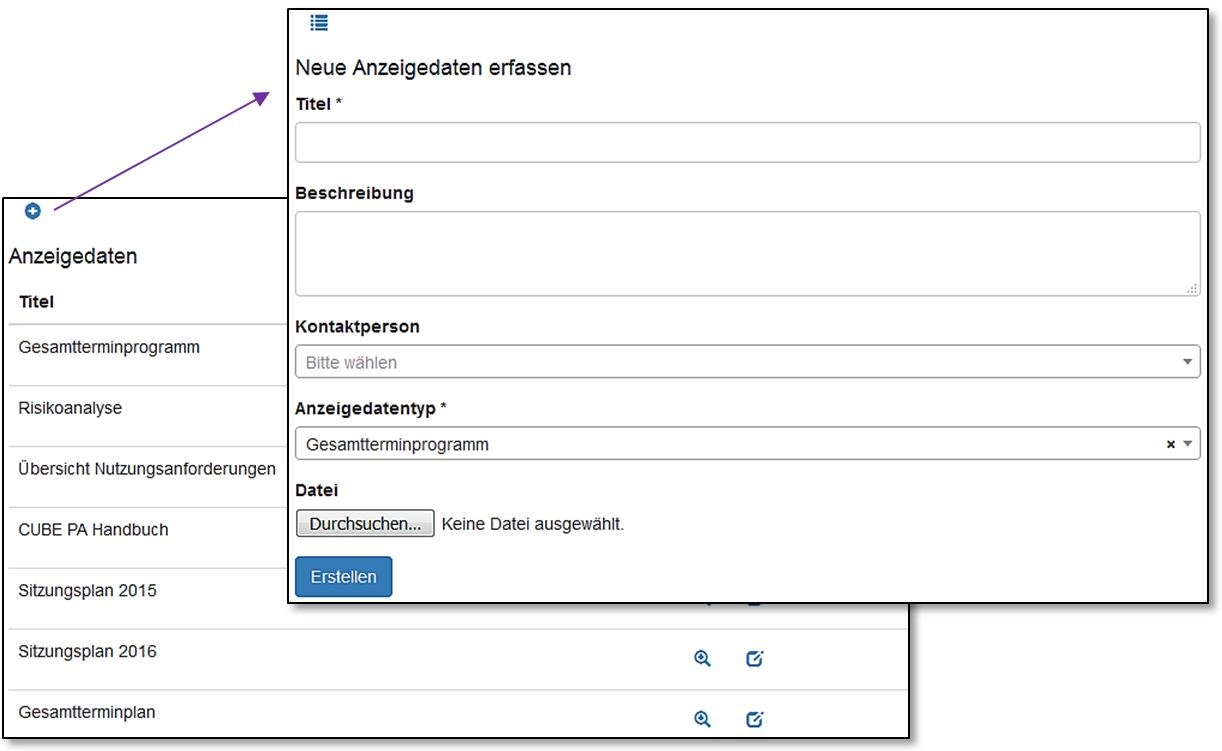
\includegraphics[width=1\linewidth]{138_AnzeigedatenErfassen.jpg}}
\caption{Saisir une nouvelle donnée d'affichage}
% \label{fig:speciation}
\end{figure}

% \small{Übersicht und Eingabemöglichkeiten für die Anzeigedatentypen und Anzeigedaten.}

\clearpage
\subsection{Listes de participants à la séance}

Des liste de participants prédéfinies pour des séances peuvent être préparées ici. Vous pouvez aussi définir si les participants choisis sont sur la liste de distribution ou pas.

\begin{figure}[H]
\center{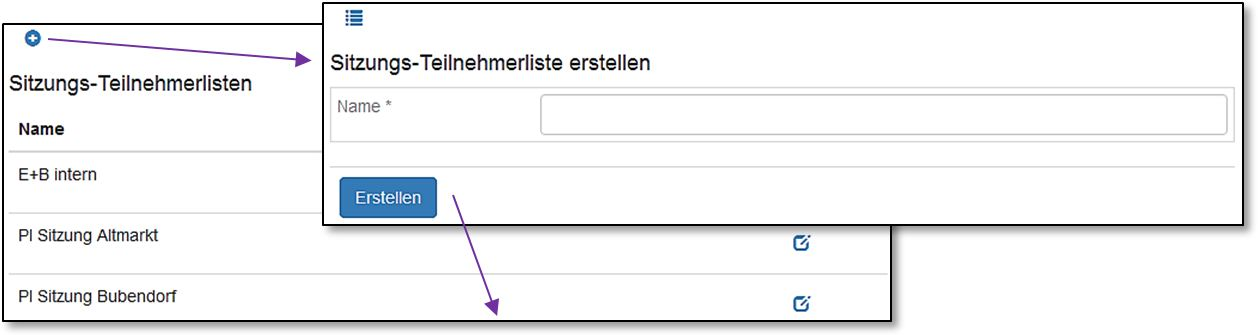
\includegraphics[width=1\linewidth]{139_SitzungsteilnehmerlistenErstellen.jpg}}
% \caption{Sitzungs-Teilnehmerlisten erstellen}
% \label{fig:speciation}
\end{figure}

\begin{figure}[H]
\vspace{-25pt}
\center{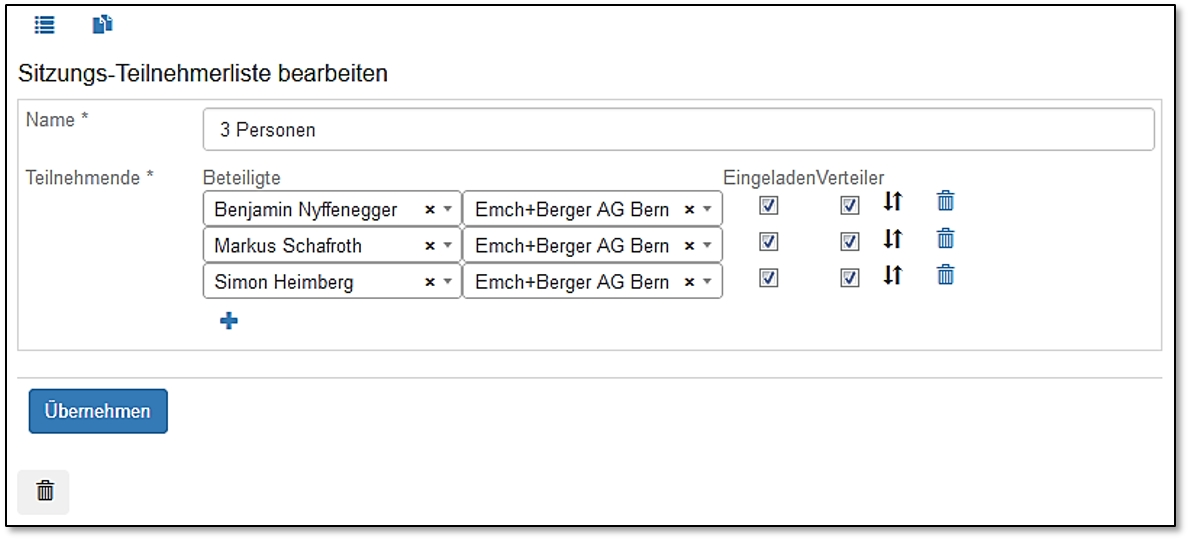
\includegraphics[width=0.75\linewidth]{../chapters/13_Konfigurationen/pictures/13-9_SitzungsteilnehmerlistenBearbeiten.jpg}}
\caption{Créer et modifier une liste de participants à une séance}
% \label{fig:speciation}
\end{figure}

Vous pouvez ajouter des participants à une liste uniquement après avoir cliqué le bouton 'Créer'. Les participants peuvent être déplacés dans la liste pour modifier leur ordre ou bien enlevés de la liste. Vous pouvez préciser si un participant à une séance est physiquement 'invité' à la séance ou s'il est uniquement sur la liste de 'distribution' du procès-verbal de la séance. Si la case 'invité' est cochée, vous pouvez alors indiquer si le participant est 'présent' ou 'absent' lorsque vous remplissez le procès-verbal de la séance. Une liste de participants à une séance peut être supprimée entièrement.

\vspace{\baselineskip}

\textbf{Copier une liste de participants à une séance :}\\
Le symbole 'copier' 
\includegraphics[height=12pt]{/Icons/kopieren.jpg} vous permet de créer une copie d'une liste de participants existante. Cliquez sur le symbole pour ouvrir la copie, qui peut être adaptée selon vos besoins. La copie comporte trois astérisques de part et d'autre de son nom, par exemple : ***Participants à la séance***.

\clearpage
\subsection{Ordres du jour standards}

Des éléments d'ordre du jour récurrents peuvent être prédéfinis ici et ensuite choisis lors de la création d'une séance.

\begin{figure}[H]
\center{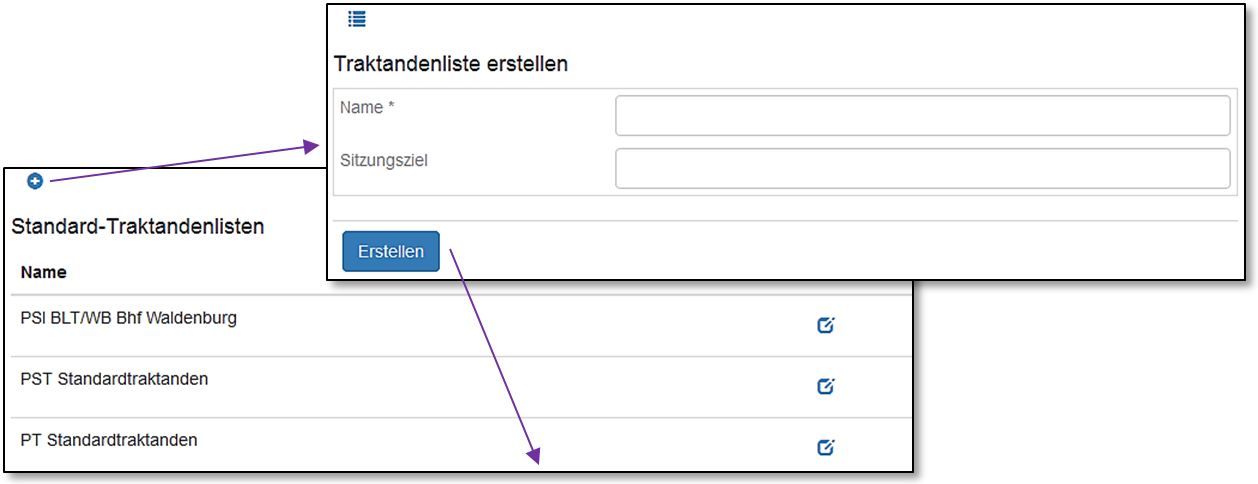
\includegraphics[width=1\linewidth]{1310_TraktandenlistenErstellen.jpg}}
\caption{Saisir un ordre du jour}
% \label{fig:speciation}
\end{figure}

\begin{wrapfigure}[14]{r}{9cm}
\vspace{-15pt}
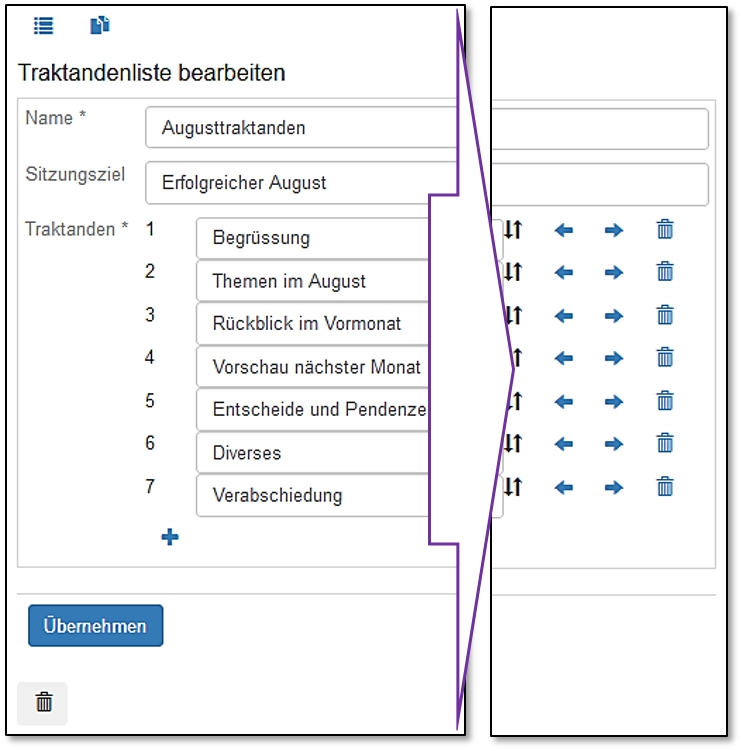
\includegraphics[height=85mm]{../chapters/13_Konfigurationen/pictures/13-10_TraktandenlistenBearbeiten.jpg}
% \caption{Status ändern}
\end{wrapfigure}

Vous pouvez ajouter des éléments à l'ordre du jour ou les modifier uniquement après avoir cliqué le bouton 'Créer'. Les nouveaux éléments d'ordre du jour peuvent être déplacés pour modifier l'ordre ou la structure (1, 2, 3 ou 2, 2.1, 3 etc.). Vous pouvez supprimer des éléments d'ordre du jour individuels ou l'ordre du jour en entier. Similairement aux listes de participants à une séance, vous pouvez créer une copie d'un ordre du jour standard en cliquant sur le symbole 'copier' 
\includegraphics[height=12pt]{/Icons/kopieren.jpg}. La copie peut être reconnue par les trois astérisques de part et d'autre de son nom (par exemple ***Ordre du jour***).
